%!TEX root = ../lectures.tex

\topic{Areas Under Curves}

We will soon have to deal a lot with sums, usually of very many (maybe infinitely many) terms, and for this we will use sigma notation, which hopefully the student is familiar with.

\begin{figure}
	\centering
	\begin{subfigure}{0.45\textwidth}
		\centering
		\begin{tikzpicture}
			\begin{axis}[
				scale = 0.6,
				axis x line = left,
				axis y line = left,
				xmin = 0,
				xmax = 5,
				ymin = 0,
				ymax = 10,
				xlabel = $x$,
				ylabel = $y$,
				xtick = {0.5, 4.5},
				xticklabels = {$a$, $b$},
				ytick = \empty,
				every axis x label/.style = {
					at = {(ticklabel* cs:1.01)},
					anchor = west,
				},
				every axis y label/.style = {
					at = {(ticklabel* cs:1.01)},
					anchor = south,
				},
				restrict y to domain = 0:10
				]
				\addplot[
				gray,
				dashed,
				samples = 200,
				pattern color = gray!60,
				pattern = north east lines,
				domain = 0.5:4.5
				]{0.5*(x+2)*sin((2*(x+2))r)+6} \closedcycle;
				\addplot[
				black,
				samples = 200,
				domain = 0.5:4.5
				]{0.5*(x+2)*sin((2*(x+2))r)+6};
				\addplot[mark=none] coordinates {(2.5, 3)} node{$A$};
			\end{axis}
		\end{tikzpicture}
		\caption{The precise area under some curve}
		\label{lec10:realarea}
	\end{subfigure}
	\begin{subfigure}{0.45\textwidth}
		\centering
		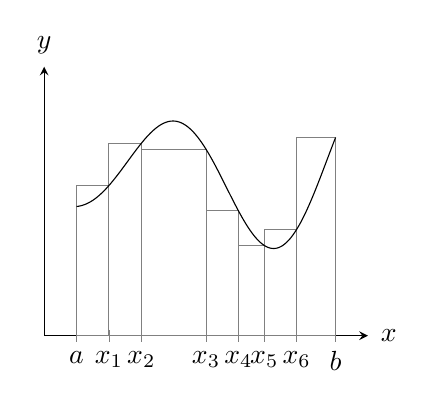
\begin{tikzpicture}
			\begin{axis}[
				scale = 0.6,
				axis x line = left,
				axis y line = left,
				xmin = 0,
				xmax = 5,
				ymin = 0,
				ymax = 10,
				xlabel = $x$,
				ylabel = $y$,
				xtick = {0.5, 1, 1.5, 2.5, 3, 3.4	, 3.9, 4.5},
				xticklabels = {$a$, $x_1$, $x_2$, $x_3$, $x_4$, $x_5$, $x_6$, $b$},
				ytick = \empty,
				every axis x label/.style = {
					at = {(ticklabel* cs:1.01)},
					anchor = west,
				},
				every axis y label/.style = {
					at = {(ticklabel* cs:1.01)},
					anchor = south,
				},
				restrict y to domain = 0:10
				]
				\addplot[
				gray,
				samples = 10,
				domain = 0.5:1
				]{5.5809} \closedcycle;
				\addplot[
				gray,
				samples = 10,
				domain = 1:1.5
				]{7.1497} \closedcycle;
				\addplot[
				gray,
				samples = 10,
				domain = 1.5:2.5
				]{6.9273} \closedcycle;
				\addplot[
				gray,
				samples = 10,
				domain = 2.5:3
				]{4.6400} \closedcycle;
				\addplot[
				gray,
				samples = 10,
				domain = 3:3.4
				]{3.3515} \closedcycle;
				\addplot[
				gray,
				samples = 10,
				domain = 3.4:3.9
				]{3.9541} \closedcycle;
				\addplot[
				gray,
				samples = 10,
				domain = 3.9:4.5
				]{7.3655} \closedcycle;
				\addplot[
				black,
				samples = 200,
				domain = 0.5:4.5
				]{0.5*(x+2)*sin((2*(x+2))r)+6};
			\end{axis}
		\end{tikzpicture}
		\caption{An approximation of the same area}
		\label{lec10:approximatearea}
	\end{subfigure}
	\caption{The area under a curve, both exact and as estimated by a sum.}
\end{figure}

Suppose we have some function $f$, and we want to find the area between $x = a$, $x = b$, the $x$-axis, and $y = f(x)$.
Now, if this region is a polygon, it's easy, but it isn't necessarily.
See, for instance, Figure \ref{lec10:realarea}.

It \emph{can} however be estimated using polygons.
We do this by \keyword{partitioning}\index{partition} (dividing) the interval $[a, b]$ into $n$ parts (not necessarily equal in length),
\[
	a = x_0 < x_1 < x_2 < \ldots < x_{n - 1} < x_n = b.
\]
Thus the smaller sections are $[x_{i - 1}, x_i]$ for all $i = 1, 2, 3, \ldots, n$.
We denote by $\Delta x_i = x_i - x_{i - 1}$ the length of these subintervals.

The point of this is that we can now approximate the area $A$ we are interested in by taking the sum of the areas of the rectangles we form as in Figure \ref{lec10:approximatearea}, namely
\[
	S_n = f(x_1) \Delta x_1 + f(x_2) \Delta x_2 + \ldots + f(x_n) \Delta x_n = \sum_{i = 1}^n f(x_i) \Delta x_i.
\]

\noindent
Of course $S_n$ is not \emph{quite} equal to $A$, since it sometimes overestimates a bit and sometimes underestimates a bit, but it seems reasonable that if we make $n$ greater, so that we're splitting the interval up into finer parts, and at the same time make sure the $\Delta x_i$ are getting smaller, then we'll approach $A$, i.e.
\[
	A = \lim_{\substack{n \to \infty \\ \max\Set{\Delta x_i} \to 0}} S_n.
\]

\begin{example}
	Find the area of the region bounded by $y = x^2$, $y = 0$, $x = 0$, and $x = b$, where $b > 0$.

	We divide the interval $[0, b]$ into $n$ equal parts, as illustrated in Figure \ref{lec10:x^2area}, each with width $\Delta x_i = b/n$.
	The height of the rectangle at $x = x_i$ is then $(i b / n)^2$, whereby\footnote{Feel free to verify on your own, perhaps by induction, that the last step is correct.}
	\[
		S_n = \sum_{i = 1}^n f(x_i) \Delta x_i = \sum_{i = 1}^n \Big ( \frac{i b}{n} \Big )^2 \frac{b}{n} = \frac{b^3}{n^3} \sum_{i = 1}^n i^2 = \frac{b^3}{n^3} \frac{n (n + 1)(2n + 1)}{6}.
	\]

	\noindent
	Taking the limit, we find that
	\[
		\lim_{n \to \infty} b^3 \frac{(n + 1)(2n + 1)}{6 n^2} = b^3 \lim_{n \to \infty} \frac{2n^2 + 3n + 1}{6 n^2} = \frac{b^3}{3} = A. \qedhere
	\]
\end{example}

\begin{figure}
	\centering
	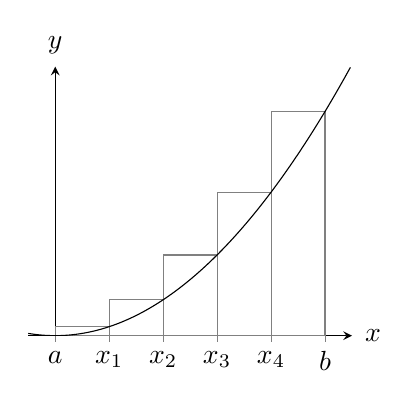
\begin{tikzpicture}
		\begin{axis}[
			scale = 0.6,
			axis x line = left,
			axis y line = middle,
			xmin = -0.5,
			xmax = 5.5,
			ymin = 0,
			ymax = 30,
			xlabel = $x$,
			ylabel = $y$,
			xtick = {0, 1, 2, 3, 4, 5},
			xticklabels = {$a$, $x_1$, $x_2$, $x_3$, $x_4$, $b$},
			ytick = \empty,
			every axis x label/.style = {
				at = {(ticklabel* cs:1.01)},
				anchor = west,
			},
			every axis y label/.style = {
				at = {(ticklabel* cs:1.01)},
				anchor = south,
			},
			restrict y to domain = 0:30
			]
			\addplot[
			gray,
			samples = 10,
			domain = 0:1
			]{1} \closedcycle;
			\addplot[
			gray,
			samples = 10,
			domain = 1:2
			]{4} \closedcycle;
			\addplot[
			gray,
			samples = 10,
			domain = 2:3
			]{9} \closedcycle;
			\addplot[
			gray,
			samples = 10,
			domain = 3:4
			]{16} \closedcycle;
			\addplot[
			gray,
			samples = 10,
			domain = 4:5
			]{25} \closedcycle;
			\addplot[
			black,
			samples = 200,
			domain = -0.5:5.5
			]{x^2};
		\end{axis}
	\end{tikzpicture}
	\caption{Estimating the area under $y = x^2$ using rectangles.}
	\label{lec10:x^2area}
\end{figure}

\noindent
We mentioned earlier that $\Delta x_i$ needn't all be equal.
Indeed, trying to use the same partition in the next problem we'd run into trouble.

\begin{exercise}
	Let $0 < a < b$, and let $k \neq -1$ be real.
	Show that the area bounded by $y = x^k$, $y = 0$, $x = a$, and $x = b$ is
	\[
		A = \frac{b^{k + 1} - a^{k + 1}}{k + 1}.
	\]

	\noindent
	Hints: Let $t = (b/a)^{1/n}$, and use the partition $x_0 = a$, $x_1 = a t$, $x_2 = a t^2$, \ldots, $x_n = a t^n = b$.

	Also recall what we know about geometric sums, i.e. that
	\[
		\sum_{i = 1}^n r^i = \frac{r^{n + 1} - 1}{r - 1},
	\]
	or maybe more useful,
	\[
		\sum_{i = 1}^n r^{i - 1} = \frac{r^n - 1}{r - 1},
	\]
	for $r \neq 1$.

	You'll also at some point change a limit to infinity to a limit at $0^+$, and use L'H\^{o}pital's rule.

	If you like, try to use the same partition as before as well, to see why this is problematic.
\end{exercise}

\topic{Definite Integrals and Riemann Sums}

In the following discussion we will assume that $f$ is continuous on the interval $[a, b]$.

Let us go back to partitions, say
\[
	P = \Set{x_0, x_1, x_2, \ldots, x_{n - 1}, x_n},
\]
such that
\[
	a = x_0 < x_1 < x_2 < \ldots < x_{n - 1} < x_n = b.
\]

\noindent
Now since $f$ is continuous on $[a, b]$, it must also be continuous on the subintervals $[x_{i - 1}, x_i]$ of $P$.
Since it is continuous on a closed interval, there must exist $\ell_i, u_i \in [x_{i - 1}, x_i]$ such that
\[
	f(\ell_i) \leq f(x) \leq f(u_i)
\]
for all $x_i \leq x \leq x_i$, by the Max-min theorem.

If we perform the same sum machinery as before with these special $\ell_i$ and $u_i$, we get areas as small and as large as possible.

\begin{definition}[Riemann sum]
	The \keyword{lower (Riemann) sum}\index{Riemann sum}\index{Riemann sum!lower}, $L(f, P)$, and the \keyword{upper (Riemann) sum}\index{Riemann sum!upper}, $U(f, P)$, for the function $f$ and the partition $P$, are
	\[
		L(f, P) = \sum_{i = 1}^n f(\ell_i) \Delta x_i, \qquad \text{and} \qquad U(f, P) = \sum_{i = 1}^n f(u_i) \Delta x_i.
	\]
\end{definition}

\begin{remark}
	If $f$ is negative, we have negative areas in our sum.
\end{remark}

\noindent
Since $L(f, P)$ is summed with the minimum for $f$ in $[x_{i - 1}, x_i]$ and $U(f, P)$ its maximum in the same interval, it is clear that
\[
	L(f, P) \leq U(f, P)
\]
for all partitions $P$.
(The only case where this might not be clear is when negative values are involved\ldots Think about it!
Draw different partitions!)

\begin{definition}[Definite integral]
	Let $f$ be a function, not necessarily continuous.
	Suppose there is exactly one number $I$ such that for \emph{every} partition $P$ of $[a, b]$ we have
	\[
		L(f, P) \leq I \leq U(f, P),
	\]
	then we say that $f$ is (Riemann) \keyword{integrable}\index{integrability} on $[a, b]$, and we call $I$ the \keyword{definite integral}\index{definite integral} of $f$ on $[a, b]$.

	We use the notation
	\[
		I = \int_a^b f(x) \, d x.
	\]

	\noindent
	Here $a$ and $b$ are called \keyword{limits of integration}, $f$ is called the \keyword{integrand}, $d x$ is called the \keyword{differential}, and $x$ is called the \keyword{variable of integration}.
\end{definition}

\noindent
Comparing this with
\[
	S_n = \sum_{i = 1}^n f(x_i) \Delta x_i,
\]
we can think of the definite integral as the sum of areas of infinitely many rectangles of height $f(x)$ and infinitesimally small widths $d x$.

We will learn next time how to efficiently calculate these sorts of quantities, but for now we close with an important theorem, the proof of which, like the Max-min theorem and the Intermediate value theorem strictly speaking doesn't belong to the course:

\begin{theorem}
	If $f$ is continuous on $[a, b]$, then $f$ is integrable on $[a, b]$.
\end{theorem}

\noindent
So far, when studying $\int\limits_a^b f(x) \, d x$, we have required $a < b$.
It turns out to be useful to drop this and allow $a = b$ and $b < a$ as well. The extension is pretty straight forward; we still have $a = x_0, x_1, \ldots, x_n = b$, but for $a = b$ they're all the same, so $\Delta x_i = 0$ (making the integral $0$), and for $b < a$ we have $\Delta x_i < 0$, so the area switches sign!

We have the following properties:

\begin{theorem}
	Let $f$ and $g$ be integrable on an interval containing $a$, $-a$, $b$, and $c$.
	Then
	\begin{romanlist}
		\item $\displaystyle \int_a^a f(x) \, d x = 0$;
		\item $\displaystyle \int_a^b f(x) \, d x = - \int_b^a f(x) \, d x$;
		\item with $A$ and $B$ constants,
		\[
			\int_a^b A f(x) + B g(x) \, d x = A \int_a^b f(x) \, d x + B \int_a^b g(x) \, d x;
		\]
		\item $\displaystyle \int_a^b f(x) \, d x + \int_b^c f(x) \, d x = \int_a^c f(x) \, d x$;
		\item if $a \leq b$, and $f(x) \leq g(x)$ for all $a \leq x \leq b$,
		\[
			\int_a^b f(x) \, d x \leq \int_a^b g(x) \, d x;
		\]
		\item (Triangle inequality), if $a \leq b$,
		\[
			\abs*{\int_a^b f(x) \, d x} \leq \int_a^b \abs{f(x)} \, d x;
		\]
		\item if $f$ is odd (i.e. $f(x) = - f(-x)$),
		\[
			\int_{-a}^a f(x) \, d x = 0;
		\]
		\item if $f$ is even  (i.e. $f(x) = f(-x)$),
		\[
			\int_{-a}^a f(x) \, d x = 2 \int_0^a f(x) \, d x.
		\]
	\end{romanlist}
\end{theorem}

\begin{proof}[(Almost literal) sketch of proof]
	\fakeitemref{1} and \fakeitemref{2} are motivated by the previous discussion.

	For \fakeitemref{3}, consider the following sketch:

	\begin{figure}[ht!]
		\centering
		\begin{subfigure}{0.3\textwidth}
			\centering
			\begin{tikzpicture}
				\begin{axis}[
					scale = 0.4,
					axis x line = left,
					axis y line = left,
					xmin = 0,
					xmax = 5,
					ymin = 0,
					ymax = 15,
					xlabel = $x$,
					ylabel = $y$,
					xtick = {0.5, 4.5},
					xticklabels = {$a$, $b$},
					ytick = \empty,
					every axis x label/.style = {
						at = {(ticklabel* cs:1.01)},
						anchor = west,
					},
					every axis y label/.style = {
						at = {(ticklabel* cs:1.01)},
						anchor = south,
					},
					restrict y to domain = 0:10
					]
					\addplot[
					gray,
					dashed,
					samples = 200,
					pattern color = gray!60,
					pattern = north east lines,
					domain = 0.5:4.5
					]{ln(x+2)+4} \closedcycle;
					\addplot[
					black,
					samples = 200,
					domain = 0.5:4.5
					]{ln(x+2)+4};
					\addplot[mark=none] coordinates {(2.5, 3)} node{Area $\alpha$};
					\addplot[mark=none] coordinates {(4, 5.79176)} node[pin=150:{$A f(x)$}]{} ;
				\end{axis}
			\end{tikzpicture}
		\end{subfigure}
		\begin{subfigure}{0.3\textwidth}
			\centering
			\begin{tikzpicture}
				\begin{axis}[
					scale = 0.4,
					axis x line = left,
					axis y line = left,
					xmin = 0,
					xmax = 5,
					ymin = 0,
					ymax = 15,
					xlabel = $x$,
					ylabel = $y$,
					xtick = {0.5, 4.5},
					xticklabels = {$a$, $b$},
					ytick = \empty,
					every axis x label/.style = {
						at = {(ticklabel* cs:1.01)},
						anchor = west,
					},
					every axis y label/.style = {
						at = {(ticklabel* cs:1.01)},
						anchor = south,
					},
					restrict y to domain = 0:10
					]
					\addplot[
					gray,
					dashed,
					samples = 200,
					pattern color = gray!60,
					pattern = north west lines,
					domain = 0.5:4.5
					]{0.5*(x+2)*sin((2*(x+2))r)+7} \closedcycle;
					\addplot[
					black,
					samples = 200,
					domain = 0.5:4.5
					]{0.5*(x+2)*sin((2*(x+2))r)+7};
					\addplot[mark=none] coordinates {(2.5, 3)} node{Area $\beta$};
					\addplot[mark=none] coordinates {(4, 4.39028)} node[pin=100:{$B g(x)$}]{} ;
				\end{axis}
			\end{tikzpicture}
		\end{subfigure}
		\begin{subfigure}{0.3\textwidth}
			\centering
			\begin{tikzpicture}
				\begin{axis}[
					scale = 0.4,
					axis x line = left,
					axis y line = left,
					xmin = 0,
					xmax = 5,
					ymin = 0,
					ymax = 15,
					xlabel = $x$,
					ylabel = $y$,
					xtick = {0.5, 4.5},
					xticklabels = {$a$, $b$},
					ytick = \empty,
					every axis x label/.style = {
						at = {(ticklabel* cs:1.01)},
						anchor = west,
					},
					every axis y label/.style = {
						at = {(ticklabel* cs:1.01)},
						anchor = south,
					},
					restrict y to domain = 0:20
					]
					\addplot[
					black,
					samples = 200,
					domain = 0.5:4.5
					]{ln(x+2)+4};
					\addplot[mark=none] coordinates {(2.5, 3)} node{Area $\alpha$};
					\addplot[
					gray,
					dashed,
					samples = 200,
					pattern color = gray!60,
					pattern = north west lines,
					domain = 0.5:4.5
					]{ln(x+2)+4+0.5*(x+2)*sin((2*(x+2))r)+7} \closedcycle;
					\addplot[
					black,
					samples = 200,
					domain = 0.5:4.5
					]{ln(x+2)+4+0.5*(x+2)*sin((2*(x+2))r)+7};
					\addplot[mark=none] coordinates {(2.5, 7.5)} node{Area $\beta$};
				\end{axis}
			\end{tikzpicture}
		\end{subfigure}
	\end{figure}

	\noindent
	For \fakeitemref{4}, at least when $a \leq c \leq b$, consider this picture:

	\begin{figure}[ht!]
		\centering
		\begin{tikzpicture}
			\begin{axis}[
				scale = 0.4,
				axis x line = left,
				axis y line = left,
				xmin = 0,
				xmax = 5,
				ymin = 0,
				ymax = 10,
				xlabel = $x$,
				ylabel = $y$,
				xtick = {0.5, 2, 4.5},
				xticklabels = {$a$, $c$, $b$},
				ytick = \empty,
				every axis x label/.style = {
					at = {(ticklabel* cs:1.01)},
					anchor = west,
				},
				every axis y label/.style = {
					at = {(ticklabel* cs:1.01)},
					anchor = south,
				},
				restrict y to domain = 0:20
				]
				\addplot[
				gray,
				dashed,
				samples = 200,
				pattern color = gray!40,
				pattern = north west lines,
				domain = 0.5:4.5
				]{0.5*(x+2)*sin((2*(x+2))r)+7} \closedcycle;
				\addplot[
				black,
				samples = 200,
				domain = 0.5:4.5
				]{0.5*(x+2)*sin((2*(x+2))r)+7};
				\addplot[
				gray,
				dashed
				] coordinates {(2, 0) (2, 7.97872)};
			\end{axis}
		\end{tikzpicture}
	\end{figure}

	\noindent
	If is isn't true that $a \leq c \leq b$, consider rearranging the same picture, and now some of the integrals will be negative because of the order of the limits of integration.

	\fakeitemref{5} is probably obvious.
	If not, consider the Riemann sums; since $f$ is bounded by $g$, so must the heights in the sums.

	\fakeitemref{6} is just \fakeitemref{5}, since $-\abs{f(x)} \leq f(x) \leq \abs{f(x)}$.
	The only remaining mystery is to prove that $\abs{f}$ must be integrable on $[a, b]$ when $f$ is (which is in fact true).

	For \fakeitemref{7} and \fakeitemref{8}, draw the appropriately symmetric pictures!
\end{proof}

\noindent
Using these properties and remembering that fundamentally they represent areas we can sometimes reduce definite integral problems to very, very simple computations.

\begin{examples}
	Calculate
	\[
		\int_{-2}^2 2 + 5 x \, d x, \qquad \int_0^3 2 + x \, d x, \qquad \text{and} \qquad \int_{-3}^3 \sqrt{9 - x^2} \, d x.
	\]

	\noindent
	We use the linearity of the integral, meaning that
	\[
		\int_{-2}^2 2 + 5 x \, d x = \int_{-2}^2 2 \, d x + \int_{-2}^2 5 x \, d x.
	\]
	The first integral in the right-hand side is just the area of a rectangle of height $2$ and width $4$, so it is $8$.
	The second integral is the integral of an odd function over a symmetric interval, whereby it is $0$, so
	\[
		\int_{-2}^2 2 + 5 x \, d x = 8 + 0 = 8.
	\]

	\noindent
	For the second one, sketch the graph and we notice that the area we're interested in is just a trapezoid, consisting of one rectangle of height 2 and width 3, on top of which is a triangle of height 3 and base 3, so
	\[
		\int_0^3 2 + x \, d x = 3 \cdot 2 + \frac{1}{2} \cdot 3 \cdot 3 = \frac{21}{2}.
	\]

	\noindent
	For the third and final one we recognise that the integrand $\sqrt{9 - x^2}$ is the expression for the upper half of a circle centred on the origin with radius 3.
	Therefore
	\[
		\int_{-3}^3 \sqrt{9 - x^2} \, d x = \frac{1}{2} \cdot \pi \cdot 3^2 = \frac{9 \pi}{2}. \qedhere
	\]
\end{examples}
